\chapter{Geometry and Physical Description}
\label{ch:geometry}

\section{Channel planform}

The fluid domain (\cref{fig:geometry}) is a channel of uniform height $h$ whose planform consists of four parts:
\begin{enumerate}
\item a straight lead-in, \SI{2}{mm} long and \SI{1}{mm} wide ($-2\le x\le0$ mm), which carries the mass-flow inlet on its upstream face;
\item the hyperbolic section $0\le x\le x_t$, whose width follows \cref{eq:intro_width} with $w_1=\SI{1}{mm}$ and $L=\SI{50}{mm}$ until it reaches $w_{\max}=\SI{10}{mm}$ at
\begin{equation}
x_t=L\left(1-\frac{w_1}{w_{\max}}\right)=\SI{45}{mm};
\label{eq:geo_xt}
\end{equation}
\item a converging section in which straight walls at \ang{45} to the axis bring the width down to \SI{1.5}{mm} at $x=\SI{49.25}{mm}$;
\item a straight outlet duct, \SI{1.5}{mm} wide and \SI{1}{mm} long, ending at $x=\SI{50.25}{mm}$, whose downstream face is the pressure outlet.
\end{enumerate}
The geometry was generated as a STEP solid by a script (\cref{app:repro}). Its fluid volume is \SI{20.745}{\milli\metre\cubed} and its planform area is \SI{143.07}{\milli\metre\squared}. Of this, the floor of the hyperbolic section, which is where cells are imaged, has an area of
\begin{equation}
A_{\mathrm{cells}}=\int_0^{x_t}w\,\dd x=w_1L\ln\frac{L}{L-x_t}=w_1L\ln\frac{w_{\max}}{w_1}=\SI{115.13}{\milli\metre\squared}.
\label{eq:geo_area}
\end{equation}
Delon \emph{et al.} evaluate the same integral for seeding, $\int_0^{4.5\,\mathrm{cm}}w\,\dd x=\SI{1.151}{cm^2}$ (their Eq.~3) \tagP. This value is reproduced exactly with $L=\SI{5}{cm}$ but not with \SI{5.3}{cm} (which gives \SI{1.002}{cm^2}), which supports the choice $L=\SI{50}{mm}$ made here. The same integral reappears as the key variable of the oxygen model (\cref{ch:o2analytical}).

The half-widths of the exported cross-sections are 0.5556, 0.7143, 1.0000, 1.6667 and \SI{5.000}{mm} at S1--S5. They equal $w(x)/2$ to four significant figures, which confirms the hyperbolic law in the meshed geometry \tagC. The \SI{2}{mm} lead-in is inferred, not documented: the pressure contour maxima exceed the centre-line pressure at $x=0$ by \SIrange{0.138}{0.143}{Pa} per \ulmin, and a \SI{2}{mm}$\times$\SI{1}{mm} lead-in predicts \SI{0.136}{Pa} per \ulmin\ (\cref{app:missing}).

\begin{figure}[htbp]
\centering
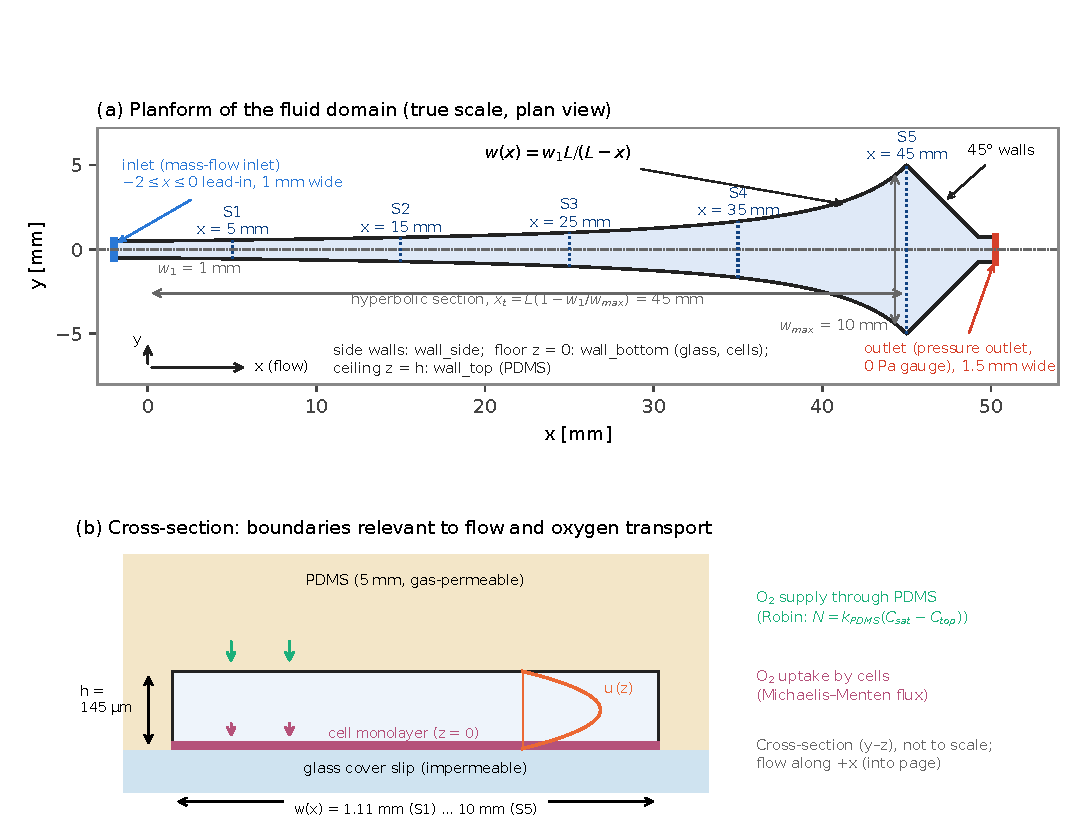
\includegraphics[width=\linewidth]{geometry_schematic.pdf}
\caption{Computational domain. (a) Planform at true scale, with the hyperbolic section, the \ang{45} converging walls, the boundaries and the five measurement stations S1--S5. (b) Schematic cross-section (not to scale). The cells sit on the glass floor ($z=0$, \texttt{wall\_bottom}); the lid and the side walls are PDMS. The oxygen fluxes drawn in (b) are used in Part B.}
\label{fig:geometry}
\end{figure}

\section{Coordinate system and boundaries}

The origin lies on the channel axis at the start of the hyperbolic section, on the floor. Here $x$ points downstream along the axis, $y$ across the width (so the side walls lie at $y=\pm w(x)/2$), and $z$ upwards across the gap ($0\le z\le h$). The mean flow is in the $+x$ direction. \Cref{tab:boundaries} lists the boundary surfaces. For the flow they are the inlet face, the outlet face and the no-slip walls. For oxygen it matters which wall is which: the cells occupy the glass floor, while the lid and the side walls are PDMS.

\begin{table}[htbp]
\centering
\caption{Boundary surfaces of the computational domain.}
\label{tab:boundaries}
\small
\begin{tabular}{@{}lll@{}}
\toprule
Surface & Location & Physical meaning\\
\midrule
\texttt{inlet} & $x=-\SI{2}{mm}$, $|y|\le\SI{0.5}{mm}$ & medium enters from the inlet port\\
\texttt{outlet} & $x=\SI{50.25}{mm}$, $|y|\le\SI{0.75}{mm}$ & medium leaves to the outlet port\\
\texttt{wall\_bottom} & $z=0$ & glass cover slip carrying the cell monolayer\\
\texttt{wall\_top} & $z=h$ & PDMS lid, \SI{5}{mm} thick\\
\texttt{wall\_side} & $y=\pm w(x)/2$ & PDMS side walls\\
\bottomrule
\end{tabular}
\end{table}

\section{Characteristic cross-sections}

\Cref{tab:stations} lists the local geometry at the stations. Two ratios control how well the analytical theory works. The first is the local aspect ratio $h/w$, which measures the influence of the side walls on the flow. It falls from 0.145 at the inlet to 0.0145 at S5. The second is the wall half-angle $\theta=\arctan[\tfrac12\,\dd w/\dd x]$, which measures how quickly the planform changes. Since
\begin{equation}
\frac{1}{2}\frac{\dd w}{\dd x}=\frac{w_1L}{2(L-x)^2},
\label{eq:geo_slope}
\end{equation}
the half-angle grows from \ang{0.57} at the inlet to \ang{6.3} at S4 and reaches \ang{45} at S5, where the diverging walls meet the converging ones. S5 is therefore not a ``slowly varying'' section. It is the corner of the planform, and this fact explains several results in \cref{ch:validation}.

\begin{table}[htbp]
\centering
\caption{Local geometry at the inlet of the hyperbolic section and at the stations ($h=\SI{145}{\micro\metre}$). $f$ is the rectangular-duct flux factor of \cref{eq:th_flux_factor}.}
\label{tab:stations}
\small
\begin{tabular}{@{}lcccccc@{}}
\toprule
Section & $x$ [mm] & $w$ [mm] & $h/w$ & $D_h$ [\si{\micro\metre}] & half-angle $\theta$ & $f(h/w)$\\
\midrule
inlet of hyperbola & 0 & 1.000 & 0.1450 & 253.3 & \ang{0.57} & 0.9086\\
S1 & 5 & 1.111 & 0.1305 & 256.5 & \ang{0.71} & 0.9178\\
S2 & 15 & 1.429 & 0.1015 & 263.3 & \ang{1.17} & 0.9360\\
S3 & 25 & 2.000 & 0.0725 & 270.4 & \ang{2.29} & 0.9543\\
S4 & 35 & 3.333 & 0.0435 & 277.9 & \ang{6.34} & 0.9726\\
S5 & 45 & 10.00 & 0.0145 & 285.9 & \ang{45} (corner) & 0.9909\\
\bottomrule
\end{tabular}
\end{table}

\section{Symmetry}

The planform is symmetric about the axis $y=0$. The flow problem is also symmetric about the mid-plane $z=h/2$, because the floor and the lid are both no-slip walls. A half or quarter model would therefore give the same flow field. The simulations nevertheless used the full domain, so the symmetry is a check on the results rather than a constraint: the shear on the floor and on the lid agrees to \SIrange{0.1}{0.8}{\percent} (\cref{sec:val_transverse}). For oxygen, the symmetry about the mid-plane is broken, because the cells consume oxygen at the floor while the lid may supply it. Only the symmetry about the axis remains.

\section{Why the dimensions matter}

The aspect ratio is small, $h/w\le0.145$, so the flow in each cross-section is close to the flow between two infinite plates. The velocity is parabolic in $z$ and almost uniform in $y$, except within about one gap height of each side wall. The shear on the floor then depends on the local width only, $\taw\propto1/w(x)$, and the hyperbolic width makes it linear in $x$. The height enters as $\taw\propto h^{-2}$ and $\Delta p\propto h^{-3}$. A \SI{3.4}{\percent} error in $h$ (\SI{145}{} instead of \SI{150}{\micro\metre}) therefore changes the shear by about \SI{7}{\percent} and the pressure drop by about \SI{11}{\percent}, which is why the height inconsistency of the reference paper matters. For oxygen, $h$ sets the diffusion time across the gap and $w(x)$ sets the area of cells fed by a given flow (\cref{ch:o2analytical}).
